\chapter{Implementace}
\label{chap:implementation}
Celý systém pro správu kampaní je rozdělen do několika celků. Základem je webový server, postavený na frameworku Next.js, který zprostředkovává komunikaci mezi dalšími častmi.
Pracovní postup se systémem je následnový:
\begin{enumerate}
    \item import dat,
    \item úprava ve webovém rozhraní,
    \item exportování dat a použití v reklamním systému.
\end{enumerate}
Data jsou perzistována v relační databázi PostgreSQL pomocí ORM systému Prisma.
Paměťové úložiště v databázi Redis slouží jako zprostředkoval pro frontu úloh, cacheování požadavků na API třetích stran a dočasné úložiště importovaných dat.

\begin{figure}[h]
    \centering
    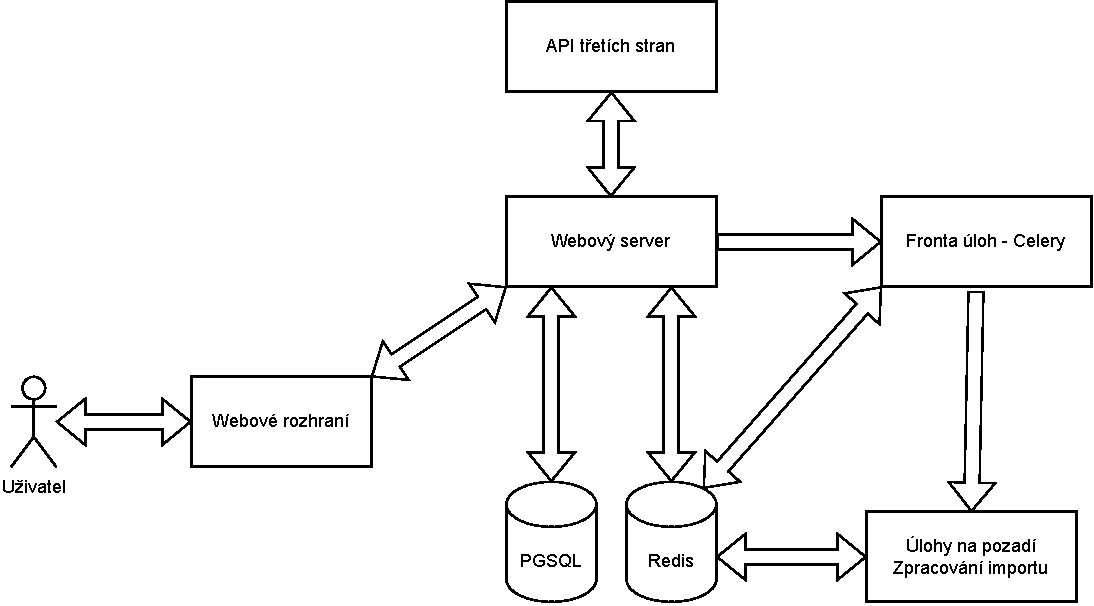
\includegraphics[width=1\textwidth]{Figures/system-overview.pdf}
    \caption{Náhled systému}
    \label{fig:system-overview}
\end{figure}

\section{Importování souborů}
Ve webovém rozhraní, které slouží jako hlavní způsob interakce systému s uživatelem, je umožněno vybírání souboru ke zpracování.
Jakmile je tento soubor nahrán na server, vytvoří se nový úkol do fronty úloh. Na pozadí je automaticky spuštěň nový proces, který
zpracovává nahraný soubor. Uživatele v tento moment nic neblokuje a nebrání s další interakcí se systémem. Jakmile jsou data ze souboru
získána, jsou dočasně uloženy do paměťové databáze Redis a uživateli je zobrazeno upozornění.
Po rozkliknutí je přesměrován na stránku, kde si může vybrat, které části si přeje importovat a které ne.
V případě využití funkce najít a nahradit se spustí další úloha na pozadí, která tento požadavek splní.
Následně jsou data zapsaná do relační databáze.

Na třídním diagramu \ref{fig:campaigns-class-diagram} je vidět struktura kampaní, do které jsou data z CSV souboru transformována. Třída \emph{Targeting} reprezentuje všechny
možné typy cílení, které se mohou v CSV vyskytovat (věk, pohlaví, \ldots). 

\begin{figure}[h]
    \centering
    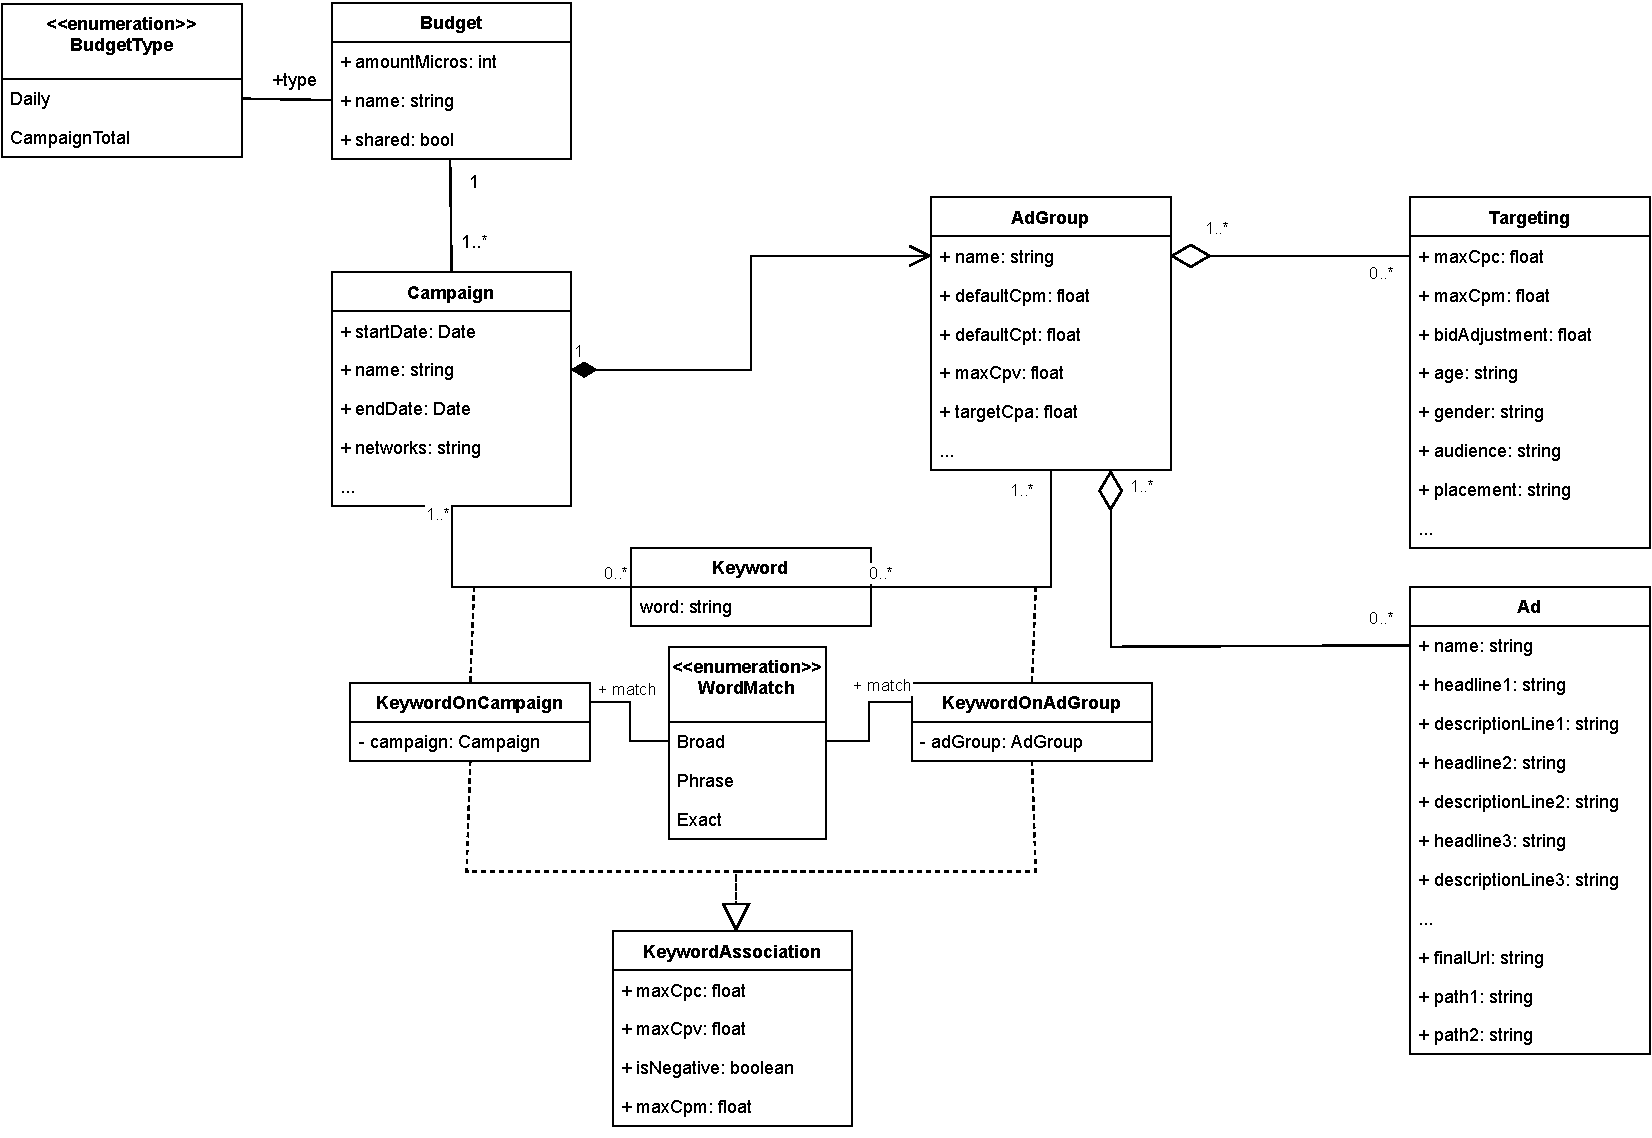
\includegraphics[width=1\textwidth]{Figures/campaigns-class-diagram.pdf}
    \caption{Třídní diagram sturktury kampaní}
    \label{fig:campaigns-class-diagram}
\end{figure}

% Dodělat do systému funkci najít a nahradit -> další celery task, který upraví data, přepíše v 
% Redisu a pošle request na Webserver, který to už uloží do DB


\section{Tabulková správa kampaní}
Jak již bylo zminěno v části \ref{subsec:edit-campaigns}, jedním z nejrychlejších způsobu editace kampaní je tabulkovým procesorem.
Proto bylo ve webovém rozhraní vytvořena možnost pracovat podobným způsobem. Obrázek \ref{fig:datagrid-window} ukazuje celkový pohled na rozhraní, ve kterém uživatel
může provádět úpravy a správu svých kampaní a metadat. Hlavní částí je komponenta \emph{DataGrid} (\ref{fig:datagrid}). Ta jako svůj vstup vyžaduje definici jednotlivých sloupců
a pak samotná data. Definice sloupců obsahuje jeho datový typ, případně taky seznam možností, ze kterých si uživatel bude moct vybrat svou požadovanou hodnotu.
Tato funkcionalita je znázorněna na obrázku \ref{fig:cell-choices} a jeji využití spočívá převážně u sloupců, jenž mají jednoznačně definované možné hodnoty.

\begin{figure}[h]
    \centering
    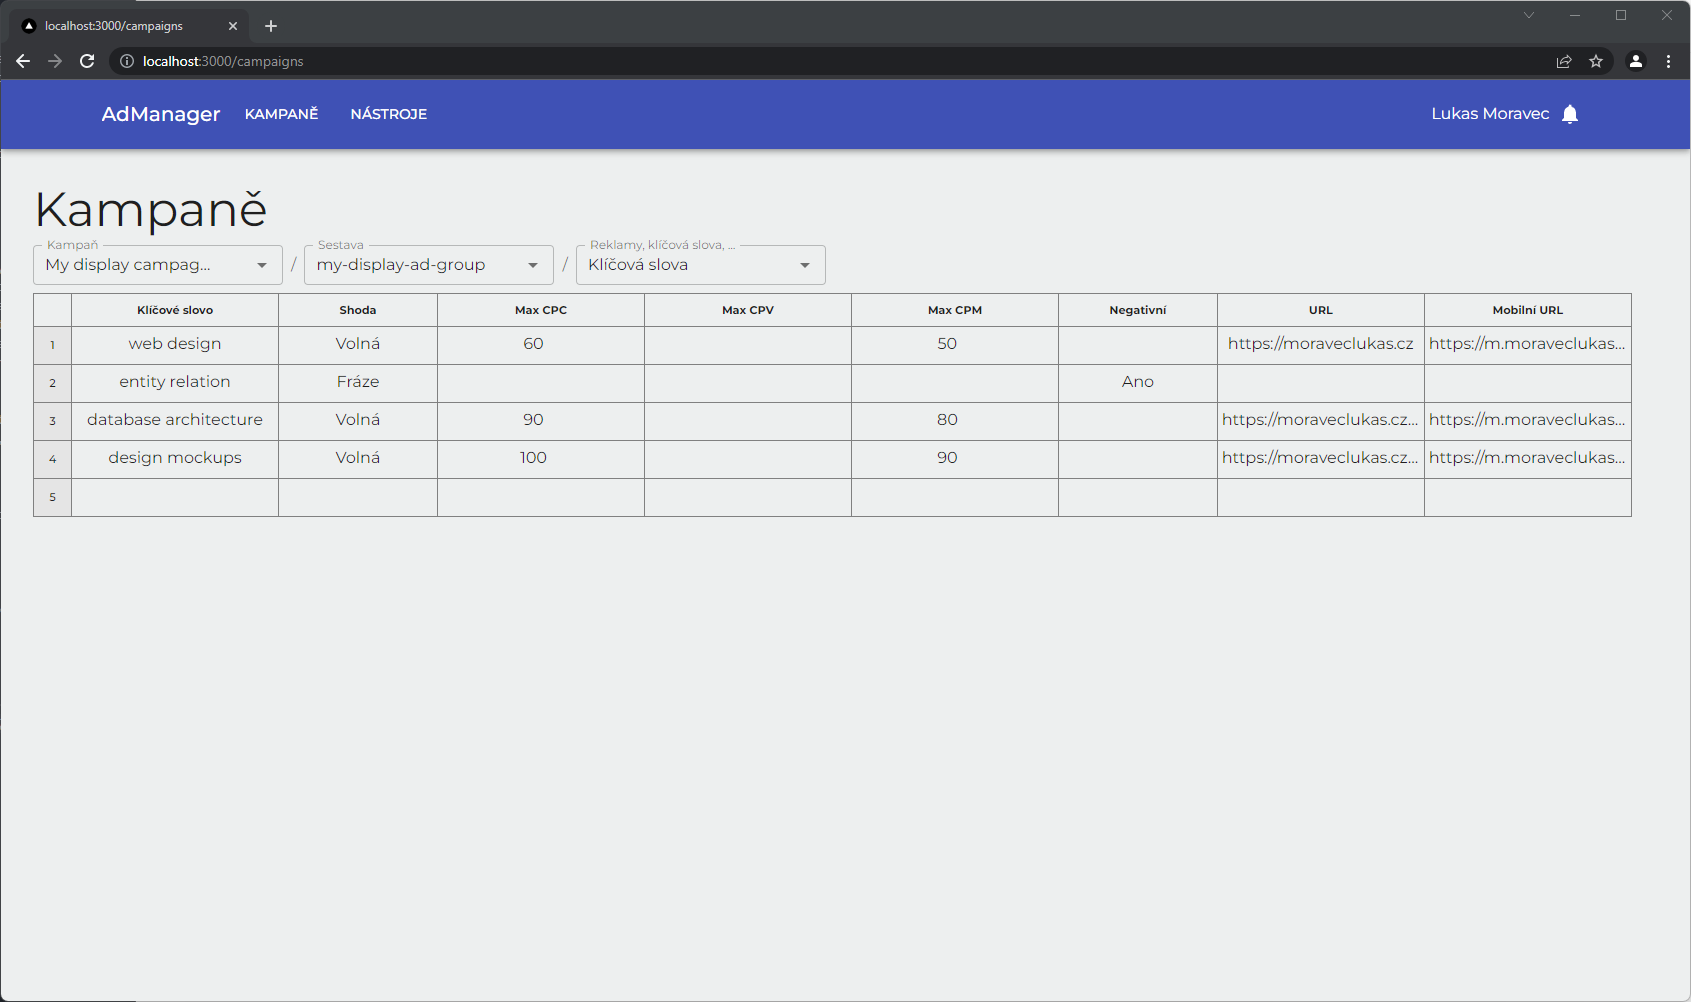
\includegraphics[width=1\textwidth]{Figures/ui/whole-window.png}
    \caption{Pohled na webové rozhraní umožňující správu kampaní}
    \label{fig:datagrid-window}
\end{figure}

\begin{figure}[h]
    \centering
    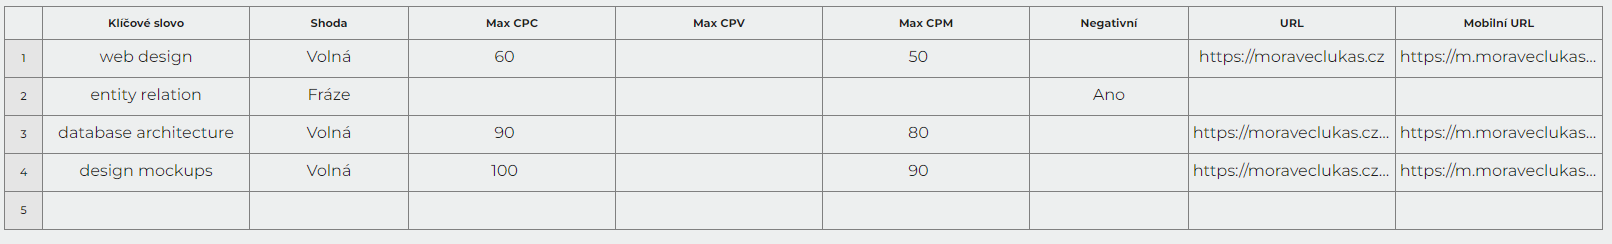
\includegraphics[width=1\textwidth]{Figures/ui/datagrid.png}
    \caption{Komponenta DataGrid}
    \label{fig:datagrid}
\end{figure}

\begin{figure}[h]
    \centering
    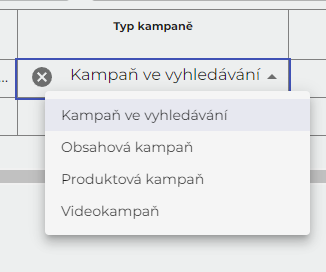
\includegraphics[width=0.5\textwidth]{Figures/ui/cell-choices.png}
    \caption{Výběr možností}
    \label{fig:cell-choices}
\end{figure}

\subsection{Automatické ukládání změn}
Všechny provedené změny se automaticky ukládají pomocí technologie \emph{Websockets}. Ta umožňuje vytvořit obousměrný komunikační kanál mezi serverem a prohlížečem uživatele.
Websocket na serverové straně také umožňuje vzniklé události přeposílat všem připojeným klientům metodou broadcast. Tato spojení lze rozlišit podle přihlášeného uživatele nebo jakýchkoli jiných
kritérií. Díky onomu přeposílání událostí je možné, aby na správně kampaní pracovalo více uživatelů najednou a v reálném čase viděli všechny prováděné změny.

\subsection{Výběr klíčových slov}
Pokud si uživatel ke svému účtu uloží API klíč k platformě Sklik, může využívat doporučování klíčových slov. Stisknutím kláves CTRL a šipky nahoru se otevře dialogové okno,
znázorněné na obrázku \ref{fig:keyword-dialog}. Zobrazí různé návrhy klíčových slov, včetně průměrné ceny za proklik při reakci na klíčové slovo a také počet zahledání, až půl roku zpětně.
Lze vybrat více klíčových slov najednou. Pokud se tak stane, vytvoří se nové záznamy klíčových slov s totožnými parametry, které měl aktuálně nastaven upravovaný záznam.  

\begin{figure}[h]
    \centering
    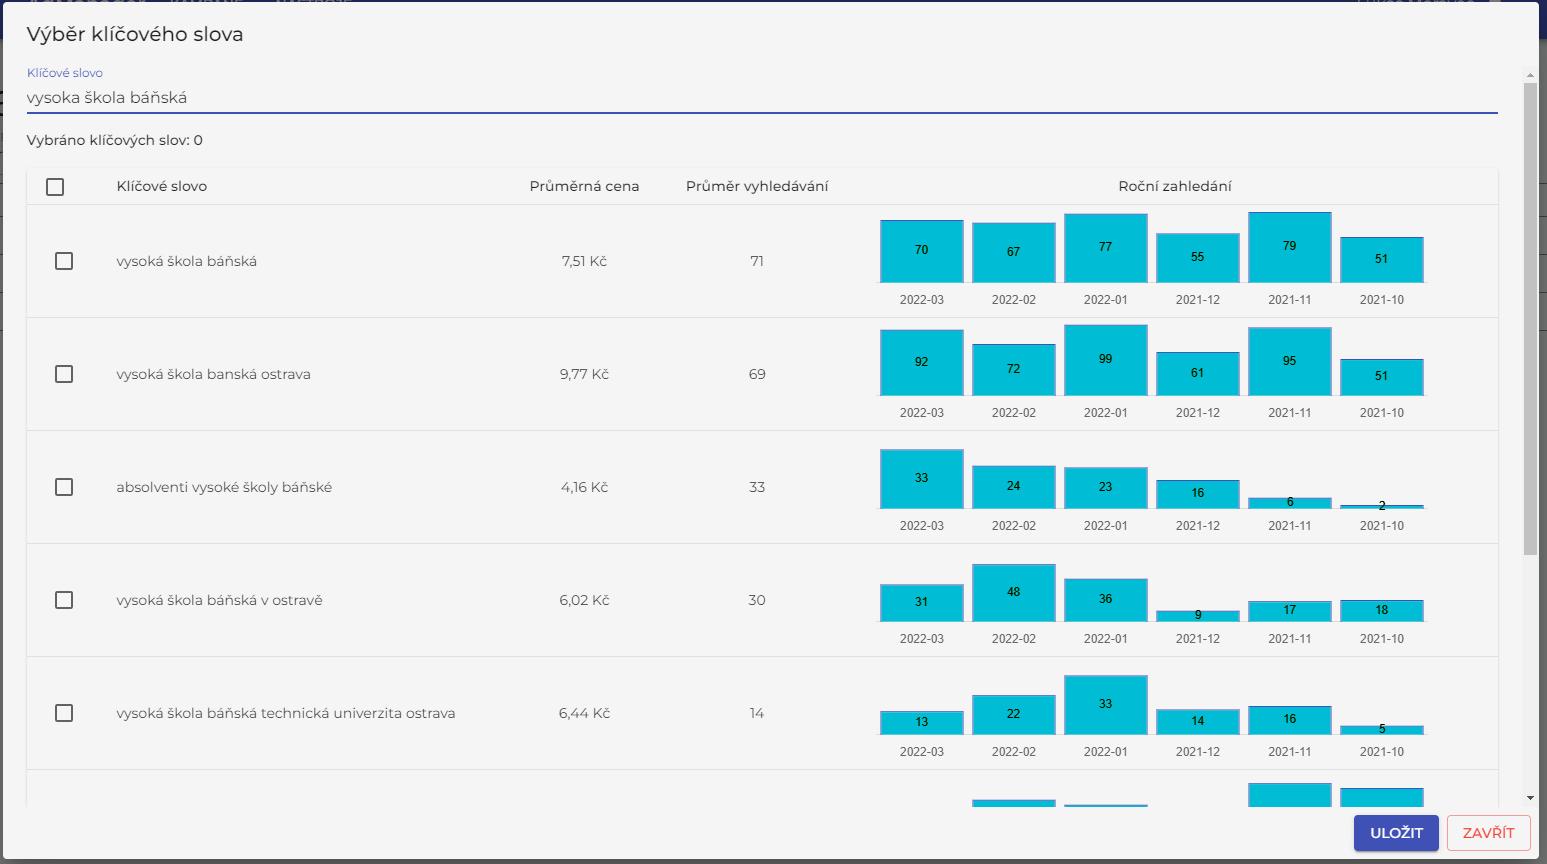
\includegraphics[width=1\textwidth]{Figures/ui/keyword-dialog.png}
    \caption{Dialogové okno pro výběr klíčových slov}
    \label{fig:keyword-dialog}
\end{figure}


\subsection{Návrhy klíčových slov}

\section{Export kampaní}


\endinput